\subsection{Data processing} \label{meth-encode-data-subsect}
The RRBS data for K562 and H1-hESC cells were produced by the Myers Lab at the HudsonAlpha Institute for Biotechnology and are available via the Gene Expression Omnibus (GEO) series GSE27584. These data were already pre-processed and aligned to the reference genome \emph{hg19}. For our analysis we used the resulting BED files. \emph{Fig. \ref{meth-dens-pic}} depicts the density of the methylation percentage in the K562 (left) and H1-hESC (right) cells. We observe that this density is bimodal for both cell types, and the majority of the CpGs are un-methylated. 

\begin{figure}[ht!]
     \begin{center}
        \subfigure[]{
            \label{meth:first}
            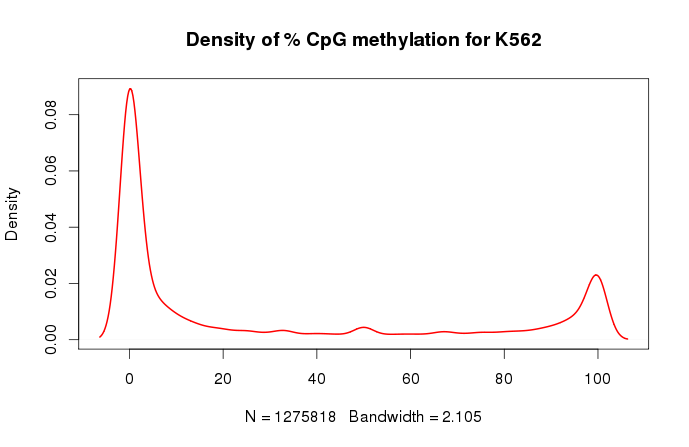
\includegraphics[width=0.47\textwidth]{images/methK562}
        }
        \subfigure[]{
           \label{meth:second}
           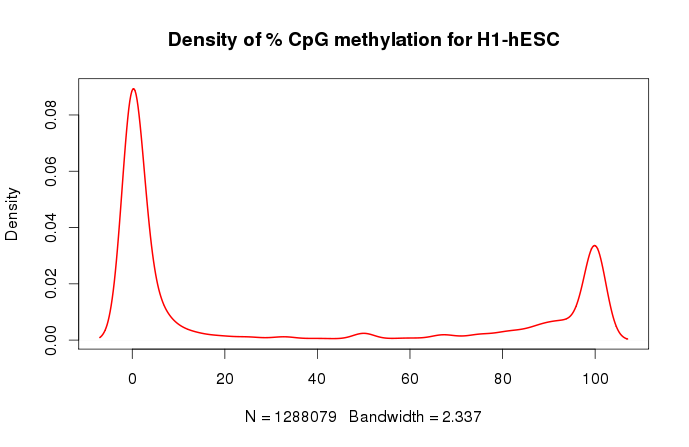
\includegraphics[width=0.47\textwidth]{images/methH1hESC}
        }
    \end{center}
    \caption{\emph{Density plot of methylation percentage in the K562 (a) and H1-hESC (b) cell lines.}}
   \label{meth-dens-pic}
\end{figure}

To investigate the relationship between DNA methylation profiles and gene expression, we used the corresponding paired-end RNA-Seq data for K562 and H1-hESC cells, produced by Caltech and are available via the GEO accession number GSE33480. The RNA-Seq data were pre-processed and mapped to the reference genome \emph{hg19} using \emph{TopHat} \citep{Trapnell2009} and gene expression quantification in FPKM were produced using \emph{Cufflinks} \citep{Trapnell2010}. Finally, the RNA-Seq data were filtered to keep only the protein-coding genes. 

For the purpose of this project, we are interested in mixture modelling methylation profiles around promoter regions. To define a promoter region, we extract Transcription Start Sites (TSS) from the RNA-Seq data, since they contain annotation data with the start sites of each gene. Then, we take $n$ base pairs upstream and downstream for each TSS, resulting in promoter regions of length $2n$ base pairs. Promoter regions that contained less than 10 CpG sites in total, were excluded from the experiments. Finally, promoter regions that had the same methylation level of CpGs in all the locations were also discarded. 

%This, was mainly done to reduce the number of un-methylated promoter regions.